\documentclass[11pt]{beamer}
\usetheme{Warsaw}
\usepackage[utf8]{inputenc}
\usepackage[english]{babel}
\usepackage{amsmath}
\usepackage{amsfonts}
\usepackage{amssymb}
\usepackage{graphicx,wrapfig,lipsum}
\usepackage{multirow}
\usepackage{tikz}


\author{Alexander Kollert\\ Babak Maser\\Sascha Wernegger}
\title{Key-Point based Image retrival under ISO still image compression standards (JPEG,JEPG2000,JPEG XR))}
%\setbeamercovered{transparent} 
%\setbeamertemplate{navigation symbols}{} 
%\logo{} 
%\institute{} 
%\date{} 
%\subject{} 

\newenvironment<>{varblock}[2][.9\textwidth]{%
  \setlength{\textwidth}{#1}
  \begin{actionenv}#3%
    \def\insertblocktitle{#2}%
    \par%
    \usebeamertemplate{block begin}}
  {\par%
    \usebeamertemplate{block end}%
  \end{actionenv}}
\begin{document}

\tikzset{
  every overlay node/.style={anchor=north west},
}
% Usage:
% \tikzoverlay at (-1cm,-5cm) {content};
% or
% \tikzoverlay[text width=5cm] at (-1cm,-5cm) {content};
\def\tikzoverlay{%
   \tikz[baseline,overlay]\node[every overlay node]
}%

\setcounter{tocdepth}{1}

\begin{frame}
\titlepage
\end{frame}

%\begin{frame}
%\tableofcontents
%\end{frame}

\section{Introduction}
	
\begin{frame}{Table of Contents}
        \tableofcontents[currentsection,currentsubsection]
\end{frame}

\subsection{Content Based Image Retrieval}
\begin{frame}{Content Based Image Retrieval}
\begin{block} {CBIR}
	\begin{itemize}
		\item \textbf{retrieval:} search images in large dataset
		\item \textbf{content based:} use image data of reference to find similar images
	\end{itemize}
\end{block}
\begin{block}{How to measure the influence of compression?}
	\begin{itemize}
		\item use retrieval system and calculate some performance measure for the results
		\item Use lossless compressed dataset and run retrieval system to calculate the performance
		\item Compress dataset to different and formats ratios and do the same
		\item interpret results
	\end{itemize}
\end{block}

\end{frame}

\subsection{Software}
\begin{frame}{Software}
\begin{block}{VlBenchmark,VLFeat}
	\begin{itemize}
		\item feature extractors
		\item retrieval system
		\item performance measure
		\item dataset
	\end{itemize}
\end{block}
\begin{block}{OpenCV}
	\begin{itemize}
		\item feature extractors
	\end{itemize}
\end{block}
\begin{block}{ImageMagick,JXRLIB}
	\begin{itemize}
		\item compression
	\end{itemize}
\end{block}
\end{frame}


\section{Performance Evaluation}

\begin{frame}{Table of Contents}
        \tableofcontents[currentsection,currentsubsection]
\end{frame}
\subsection{Recall Precision}
\begin{frame}{Recall Precision}

\begin{itemize}
	\item \textbf{Precision:} $ |\textbf{relevant documents}\cap\textbf{retrieved documents}| \over |\textbf{relevant documents}|$
	\item \textbf{Recall:} $ |\textbf{relevant documents}\cap\textbf{retrieved documents}| \over |\textbf{retrieved documents}|$
\end{itemize}

		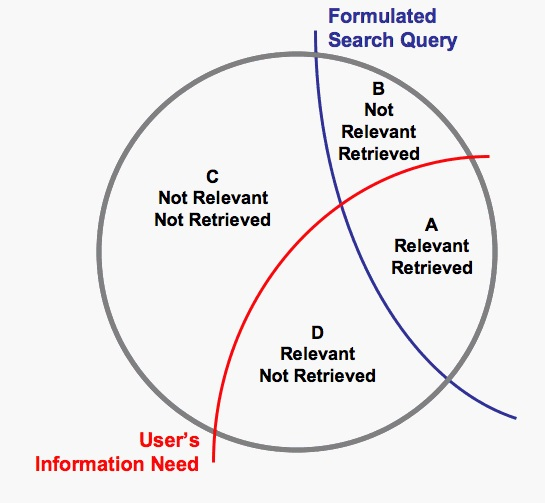
\includegraphics[width=0.5\textwidth]{img/RecallPrecision.jpg}

\end{frame}

\begin{frame}{Recall Precision}

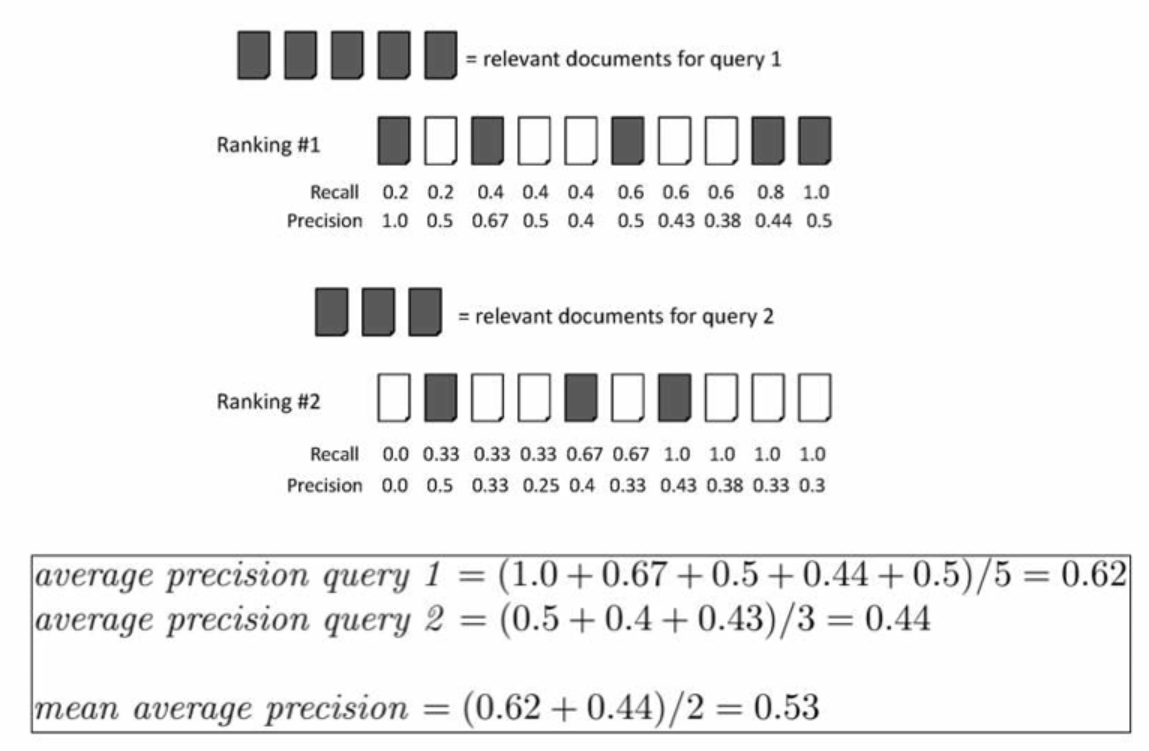
\includegraphics[width=0.9\textwidth]{img/map.png}

\end{frame}


\begin{frame}{Precision Recall Curves}
\begin{wrapfigure}{tr}{6.5cm}
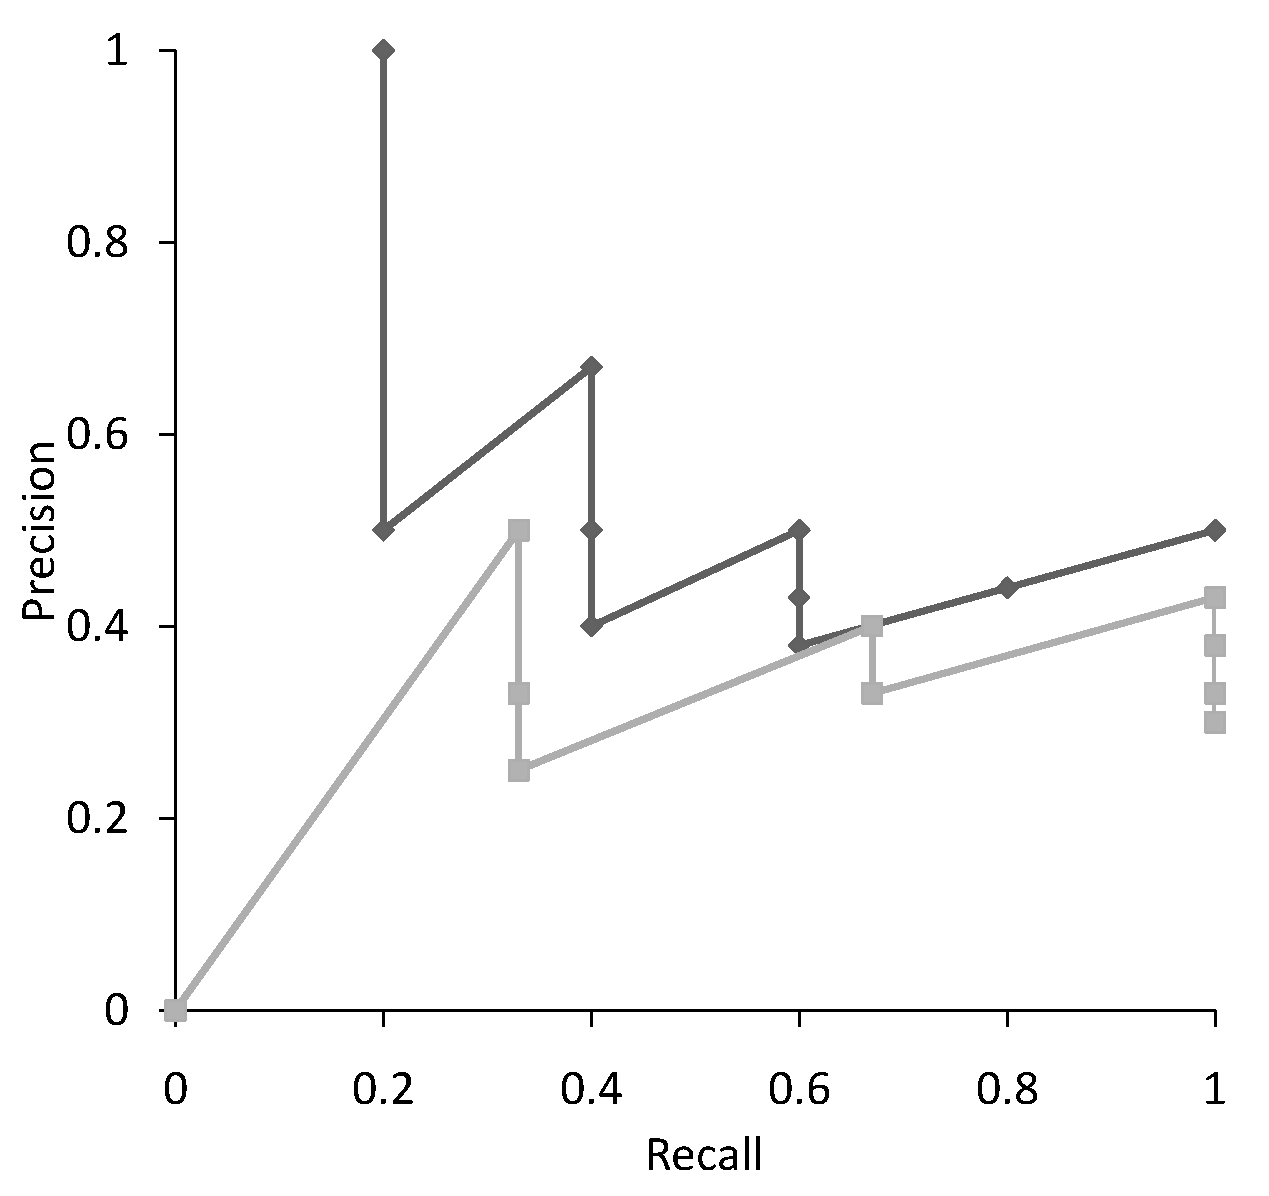
\includegraphics[width=5cm]{img/multi_prc.png}
\end{wrapfigure} 

To visualize precision and recall, we plot precision over recall.\\
If we have many queries, it is easier to interpret an averaged interpolated precision recall curve
\end{frame}

\begin{frame}{Interpolate PRC}
\begin{tabular}{ll}
\multirow{5}{*}{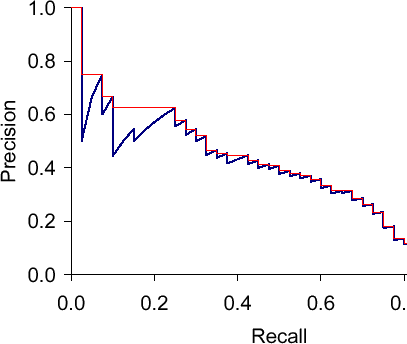
\includegraphics[width=0.45\textwidth]{img/prc.png} }
&Calculate precision at each\\
&recall level R as the\\
&maximum precision observed\\
&in any recall-precision point\\
&at a higher recall level
\end{tabular}
\end{frame}

\begin{frame}{Interpolate PRC}
\begin{wrapfigure}{tr}{6.5cm}
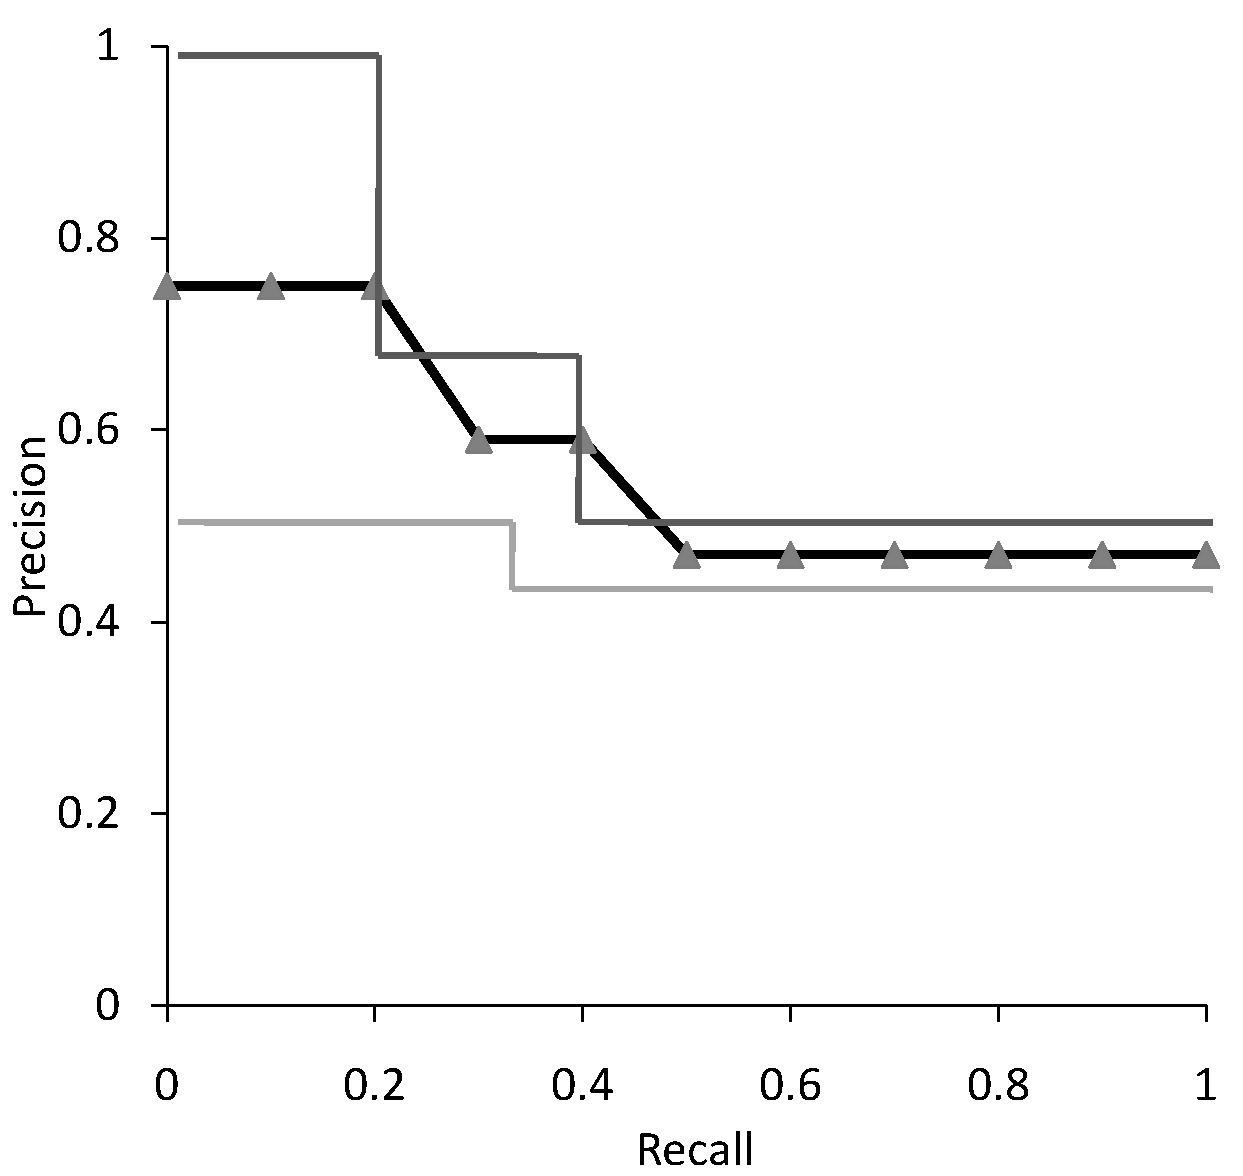
\includegraphics[width=5cm]{img/prc_average.png}
\end{wrapfigure} 
Calculate precision at each
recall level R as the
maximum precision observed
in any recall-precision point
at a higher recall level
\end{frame}

\subsection{Mean Average Precision}

\begin{frame}{Mean Average Precision}

\begin{wrapfigure}{l}{6.2cm}
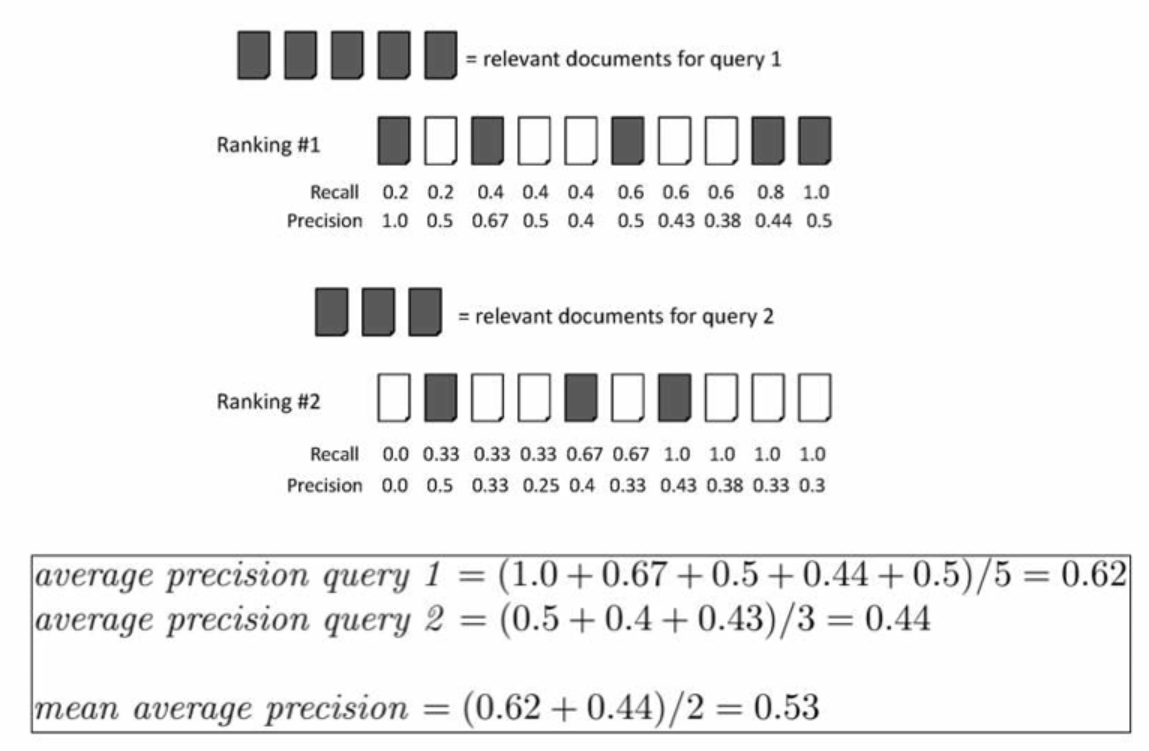
\includegraphics[width=6.5cm]{img/map.png} 
\end{wrapfigure}
\textbf{average precision} of a query is the average precision from all relevant documents.\\
\textbf{mean average precision} is the average of the query average Prexision.
\end{frame}


\section{Experiment Setup}

\begin{frame}{Table of Contents}
        \tableofcontents[currentsection,currentsubsection]
\end{frame}

\subsection{Dataset}
\begin{frame}{Dataset}
\begin{block} {Oxford Buildings Dataset}
	\begin{itemize}
		\item 5062 images
		\item compressed loss-less or with minimal loss in JPEG
		\item collected from Flickr by searching for particular Oxford landmarks
		\item manually annotated to generate ground truth for 11 different landmarks
		\item 5 queries per landmark
		\item total of 55 queries
	\end{itemize}
\end{block}
	Random sampled subsets to limit compression and benchmark speed!
\end{frame}


\begin{frame}{Queries}
	The query consists of a reference image and 4 query sets:
	\begin{itemize}
		\item [good] A nice, clear picture of the object
		\item [ok] More than 25\% of the object is clearly visible.
		\item [junk] Junk Less than 25\% of the object is visible, or there are very high levels of occlusion or distortion.
		\item [bad]  Object not present
	\end{itemize}
	\begin{tabular}{ll}
		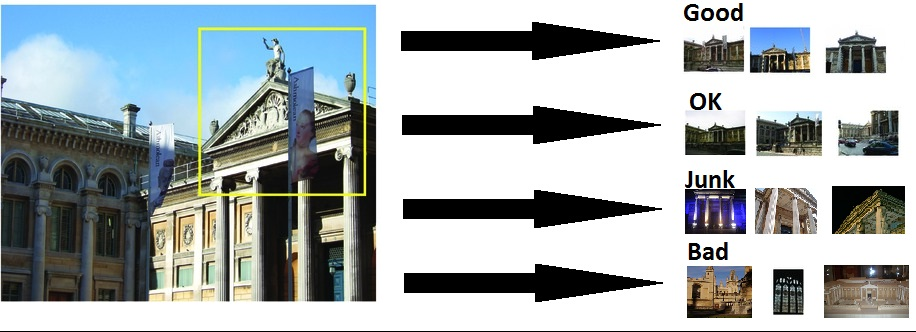
\includegraphics[width=0.7\textwidth]{img/query.jpg}
	\end{tabular}
\end{frame}


\begin{frame}{Mean Average Precision add}
VlBenchmark uses a slightly different scheme, but the calculation stays the same.
	\begin{block}{How use the four query classes}
		\begin{itemize}
			\item good and ok images are relevant
			\item junk will be ignored
			\item bad will count as wrong
		\end{itemize}
	\end{block}
Junk images do not influence precision or recall!
\end{frame}


\subsection{Compression}
\begin{frame} {Estimate Compression Ratio}
Because the dataset we used was JPEG compressed we first estimated the compression ratio.
			\begin{block}{t}	
				$s$ : avg size = 391.659 bytes.\\
				$p$ :  avg pixels = 765.969 pixel.\\
				$bpp$ : byte per pixel = 3.\\
				$r$ : avg raw size = $p*bpp$ = 2297908.\\
				$e$ : estimated ratio = $r/s = 5.867$.
			\end{block}	
			So we have a ratio smaller 6.
\end{frame}

\begin{frame}
	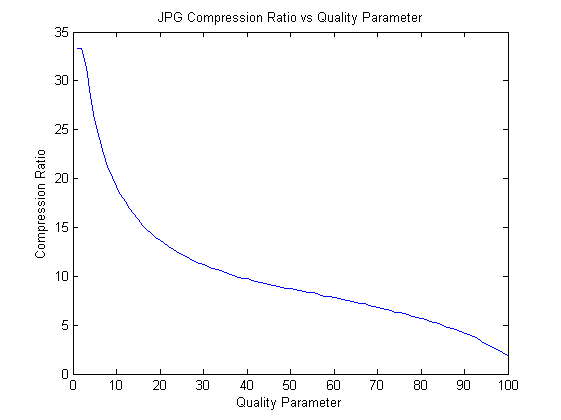
\includegraphics[width=0.8\textwidth]{img/jpg-ratio.png}
\end{frame}

\begin{frame}{Compression}
Achieved compression ratio compared to the original(391.659 bytes). 
\begin{tabular}{|l||c|c|c|}
\hline
& jpg & jxr & jp2 \\
\hline
min avg size in bytes & 13229 & 1756 & 511 \\
\hline
\end{tabular}
\begin{figure}
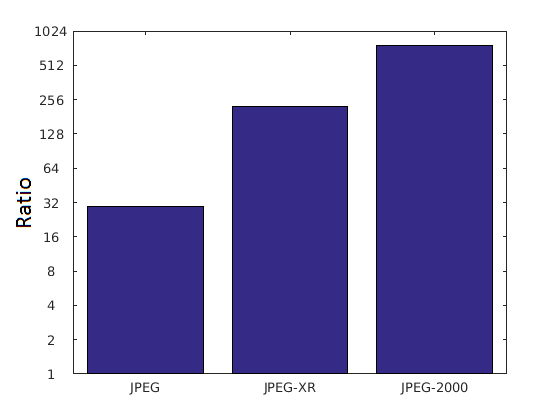
\includegraphics[width=0.6\textwidth]{img/compression.png}
\end{figure}
\end{frame}

\begin{frame}{Sample}
	\begin{figure}
		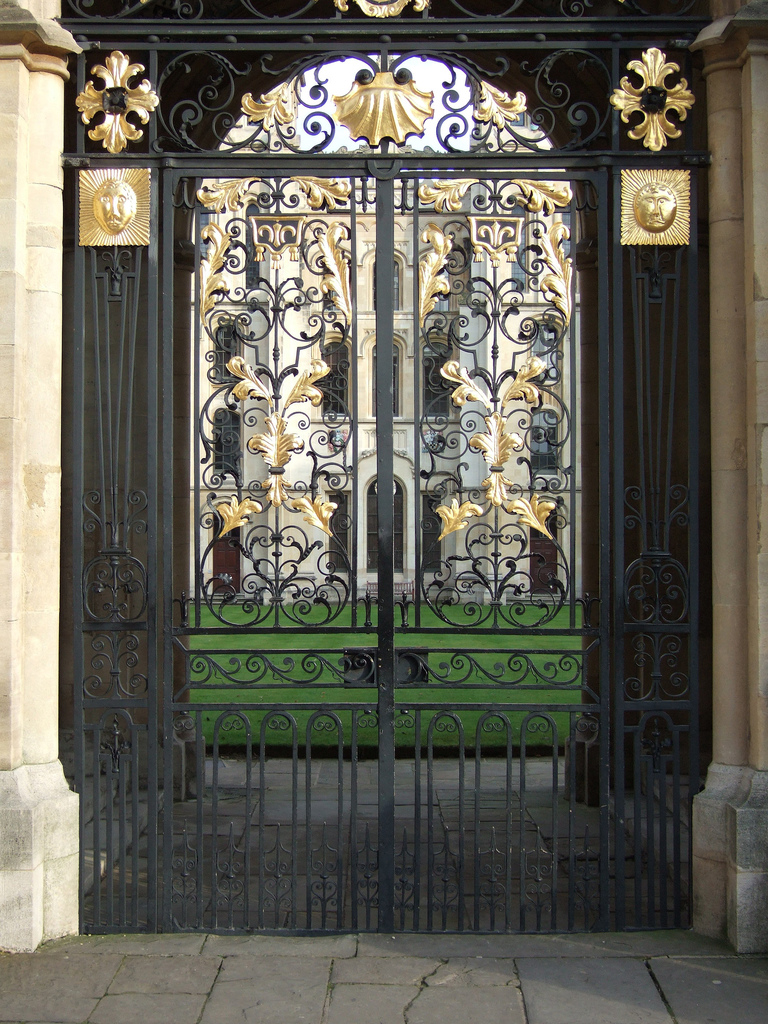
\includegraphics[width=0.5\textwidth]{img/jpg_100.jpg}
	\end{figure}
\end{frame}



\begin{frame}{Comparison}
\begin{tabular}{ccc}
	 jpg & jxr & jp2 \\ 
		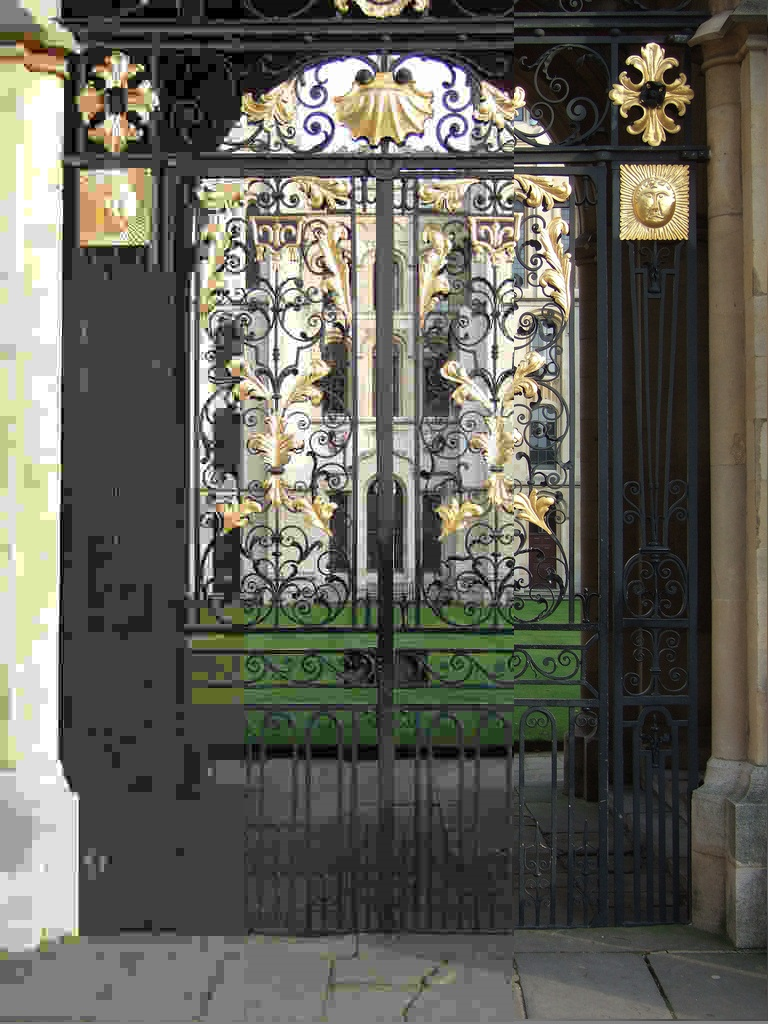
\includegraphics[width=0.3\textwidth]{img/jpg.jpg}&
		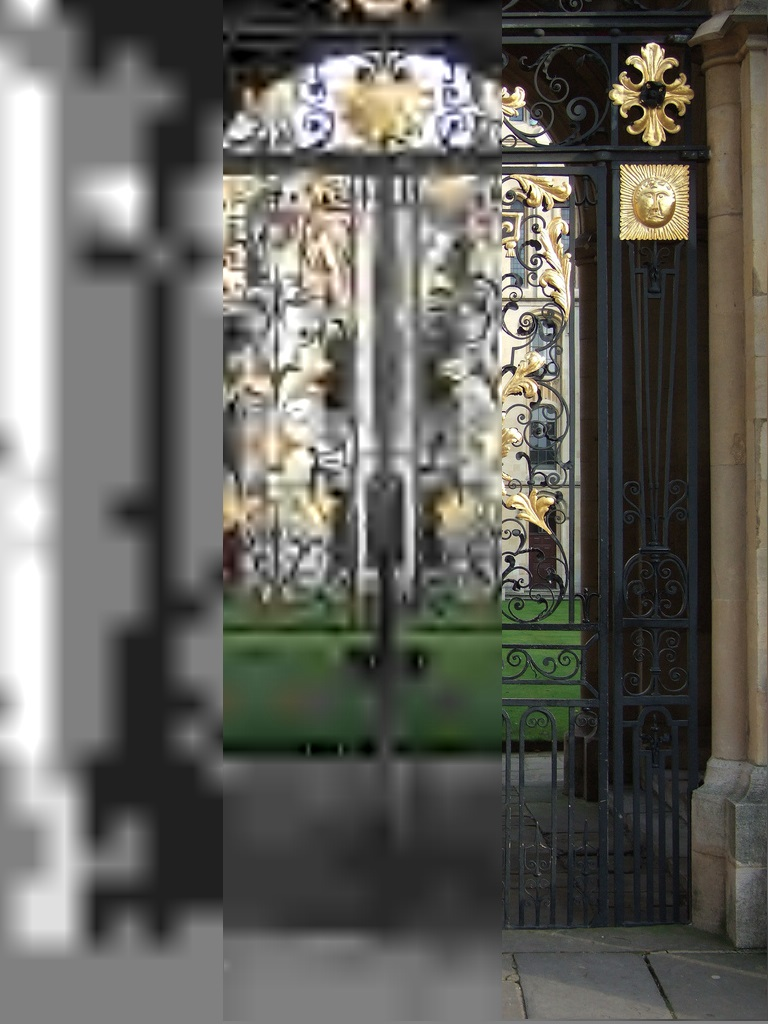
\includegraphics[width=0.3\textwidth]{img/jp2.jpg}&
		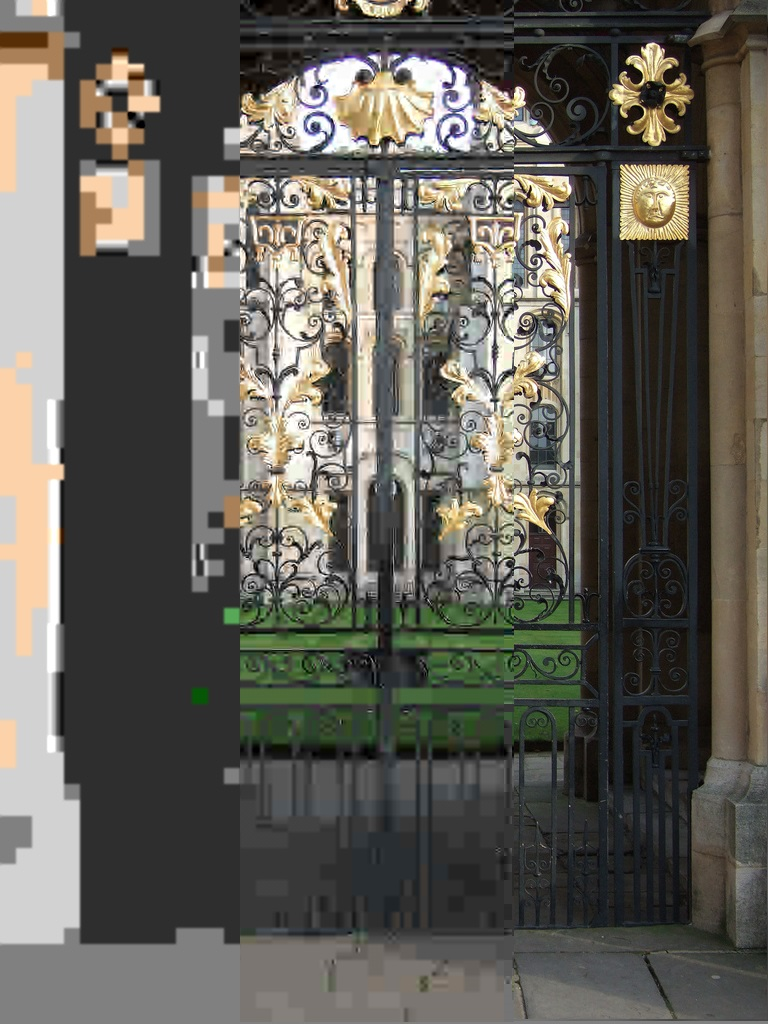
\includegraphics[width=0.3\textwidth]{img/jxr.jpg}\\
\end{tabular}
\end{frame}

\subsection{Retrieval System}

\begin{frame} {Generic Local Feature Extractor}
The Ranking in VlBenchmark is done using Local Feature Extractors. The purpose of the Feature Extractor is to calculate frames and corresponding descriptors from the image data.
	\begin{block}{Local Feature Frames}
		\begin{itemize}
			\item search image for interest points
			\item define a frame for that point(points,circles,elipses)
		\end{itemize}
	\end{block}	 
	\begin{block}{Descriptor}
		\begin{itemize}
			\item compute descriptor using the image data defined by the sframe
			\item every descriptor is a vector of same dimension
		\end{itemize}
	\end{block}
	So we got n frames and n descriptors
\end{frame}

\begin{frame} {Retrieval System}
	\begin{block}{Ranking}
		\begin{itemize}
			\item calculate reference descriptor
			\item calculate KNN's of the query descriptors
			\item for every Descriptor of the KNN's Vote for the corresponding image of the descriptor
			\item repeat for all reference descriptors
			\item Rank images by their recieved votes
		\end{itemize}
	\end{block}
		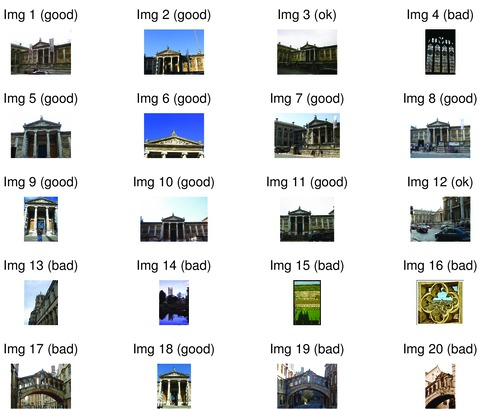
\includegraphics[width=0.5\textwidth]{img/retrieved.jpg}
\end{frame}


\section{Feature Detectors}

\begin{frame}{Table of Contents}
        \tableofcontents[currentsection,currentsubsection]
\end{frame}

\subsection{SIFT}
\begin{frame}{SIFT (Scale-Invariant Feature Transform)}
  \begin{itemize}
  \item SIFT Algorithm is comprised by 3 steps:
    \begin{enumerate}
    \item Extracting key points (features)
      \begin{enumerate}
      \item Local extrema detection
      \item Accurate keypoint localization
      \item Orientation assignment
      \end{enumerate}
    \item Feature descriptor (based on Gradient Histogram)
    \item Feature matching
    \end{enumerate}
  \end{itemize}
\end{frame}

%% \begin{frame} {Extracting key points (feature) / Detection of scale-space extrema}
%%   \begin{enumerate}
%%   \item Local extrema detection: \\
%%     \small
%%     The first stage of computation searches over all scales and image locations. It is implemented efficiently by using a difference-of-Gaussian (DoG) function to identify potential interest points that are invariant to scale and orientation.
%%     \normalsize
%%   \item Accurate keypoint localization
%%   \item Orientation assignment
%%   \end{enumerate}
%% \end{frame}

\begin{frame}{Local extrema detection}
  \begin{itemize}
  \item Find the points, whose surrounding patches (with some scale) are distinctive
  \item An approximation to the scale-normalized Laplacian of Gaussian 
    %% \( L(x,y,\sigma) = G(x,y,\sigma) * I(x,y) \) \\
    %% \( G(x,y,\sigma) = \frac{1}{2\pi\sigma^2}e^{-(x^2+y^2)/2\sigma^2} \) \\
    %% \( D(x,y,\sigma) = (G(x,y,k\sigma) - G(x,y,\sigma) - G(x,y,\sigma)) * I(x,y) = L(x,y,k\sigma) - L(x,y,\sigma) \) \\
    %% \vfill
    %% \tiny{
    %%   L is blur Image \\
    %%   G is Gaussian Blur operator \\
    %%   I is an Image \\
    %%   x,y are the location coordination \\
    %%   \(\sigma \) is Scale parameter. The amount of blur (greater value, greater the blur) \\
    %%   The * is the convolution operation in x and y. It applies Gaussian blur G onto the image I
    %% }
  \end{itemize}
\end{frame}


\begin{frame}{Difference of Gaussian}
  \begin{enumerate}
  \item A = Convolve image with vertical and horizontal 1D Gaussians, \( \sigma = \sqrt{2} \)
  \item B = Convolve A with vertical and horizontal 1D Gaussians, \( \sigma = \sqrt{2} \)
  \item DoG (Difference of Gaussian) = A – B
  \item Downsample B
  \end{enumerate}
\end{frame}

\begin{frame}{Difference of Gaussian}
  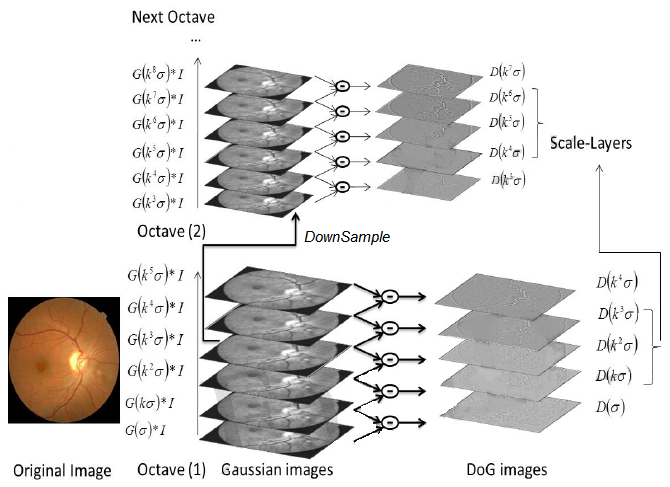
\includegraphics[width=\textwidth,height=0.9\textheight]{img/DoG.png}
\end{frame}

\begin{frame}{Accurate keypoint localization}
  \begin{columns}
    \begin{column}{.5\textwidth}
      \begin{itemize}
      \item Compare a pixel (x) with 26 pixels in current and adjucent scales (Green Circles)
      \item Scale a pixel (X) if larger/smaller than all 26 pixels
 	  \item Eliminating the Edge Response
  	  \item Eliminating poor contrast points
      \end{itemize}
    \end{column}
    \begin{column}{.5\textwidth}
      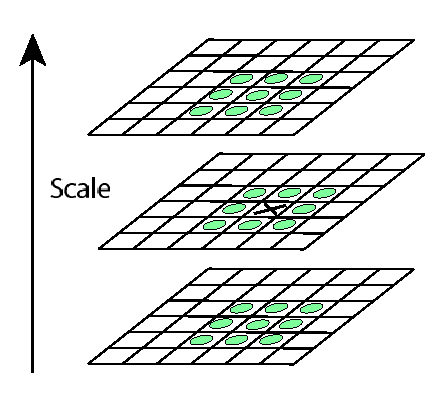
\includegraphics[width=0.8\textwidth]{img/key_localization.jpg}
    \end{column}
  \end{columns}
\end{frame}


\begin{frame}[t]{Orientation Assignment}
\begin{block}{For each remaining key point}
  Choose surrounding N x N window at DOG level it was detected  (Size of the window:The window size is equal to the size of the kernel for Gaussian Blur of amount $1.5*sigma$).  
\end{block}
  \tikzoverlay at (0cm,0.5cm) {
  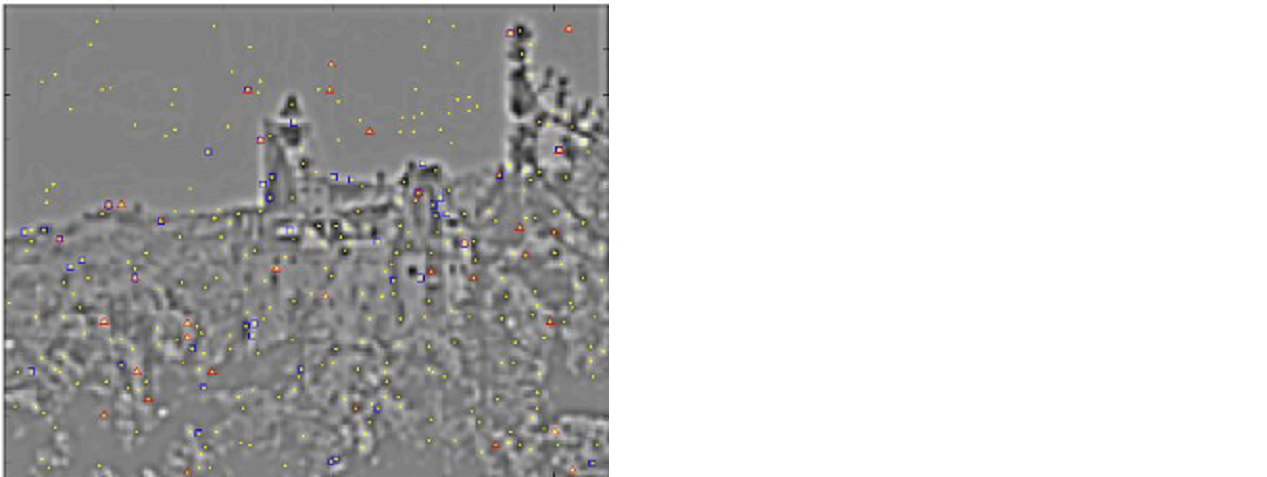
\includegraphics[scale=0.3]{img/keypoints.png}
  };
\end{frame}

\begin{frame}[t]{Orientation Assignment}
\begin{block}{For each remaining key point}
  Choose surrounding N x N window at DOG level it was detected  (Size of the window:The window size is equal to the size of the kernel for Gaussian Blur of amount $1.5*sigma$).  
\end{block}[t]
  \tikzoverlay at (0.1cm,0.5cm) {
  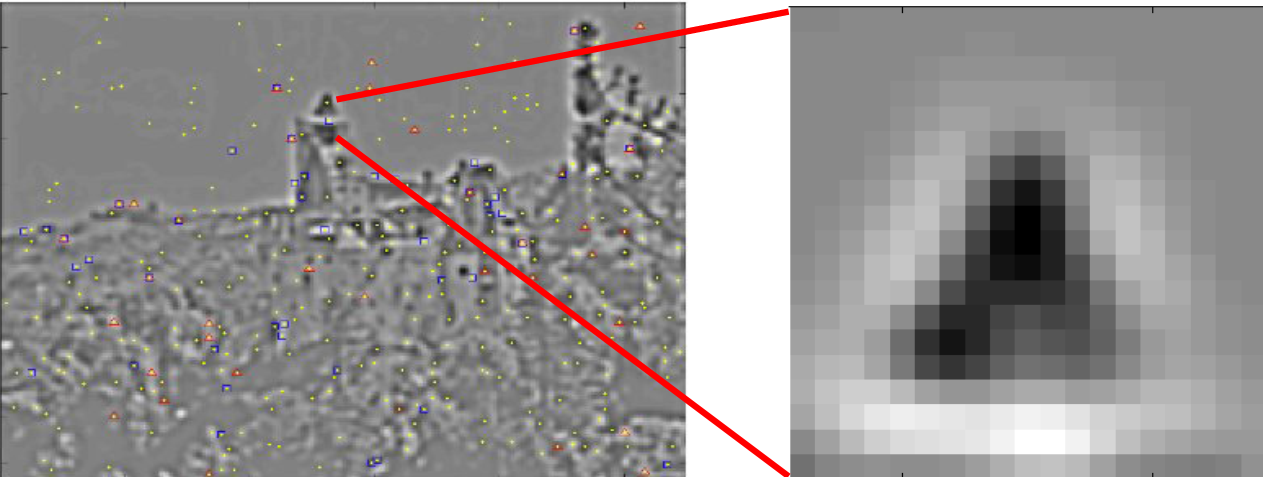
\includegraphics[width=8.8cm,height=3.8cm]{img/window.png}
  };
\end{frame}

\begin{frame}{Orientation Assignment}
  \begin{itemize}
  \item A histogram is created for mentioned images (Gradient Orientation and Weighted Magnitude)
  \item In this histogram, the 360 degrees of orientation are broken into 36 bins (each 10 degrees). Once you've done this for all pixels around the keypoint, the histogram will have a peak at some point
  \item Also, any peaks above 80\% of the highest peak are converted into a new keypoint. This new keypoint has the same location and scale as the original. But it's orientation is equal to the other peak
  \item So, orientation can split up one keypoint into multiple keypoints
  \end{itemize}
\end{frame}

\begin{frame} {Orientation Assignment}
  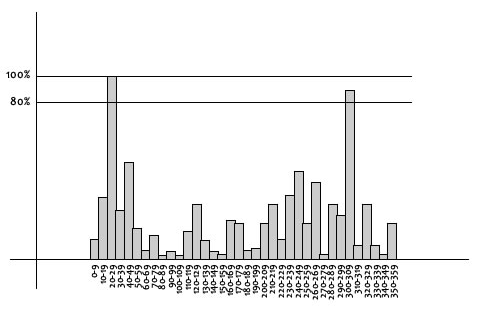
\includegraphics[width=.8\textwidth]{img/histogramOrientation.png}
\end{frame}

\begin{frame}{Orientation Assignment}
 \begin{columns}
    \begin{column}{.5\textwidth}
    	\begin{tabular}{c}
    		Gradient Magnitude\\
    		$m(x,y)=\sqrt{(L(x+1,y)-L(x-1,y)^2)}$\\ $\overline{+(L(x,y+1)-L(x,y-1))^2}$\\
      		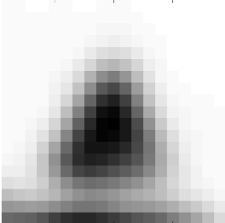
\includegraphics[width=0.5\textwidth]{img/gradient.png}\\
    		Gradient Orientation\\
    		$\theta(x,y) = \tan^{-1} (\frac{L(x,y+1)-L(x,y-1)}{L(x+1,y)-L(x-1,y)})$
    	\end{tabular}
    \end{column}
    \begin{column}{.3\textwidth}
    	\begin{tabular}{c}
    	   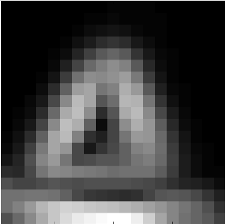
\includegraphics[width=\textwidth]{img/gradmag.png}\\
    	   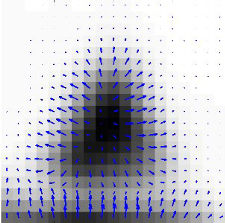
\includegraphics[width=\textwidth]{img/gradorientation.png}
    	\end{tabular}
    \end{column}
  \end{columns}
\end{frame}

\begin{frame} {Orientation Assignment}
	\begin{itemize}
		\item A histogram is created for mentioned images (Gradient Orientation and Weighted Magnitude).
		\item In this histogram, the 360 degrees of orientation are broken into 36 bins (each 10 degrees). 
		\item Once you've done this for all pixels around the keypoint, the histogram will have a peak at some point.
		\item Also, any peaks above 80% of the highest peak are converted into a new keypoint. This new keypoint has the same location and scale as the original. But it's orientation is equal to the other peak.
		\item \textbf{So, orientation can split up one keypoint into multiple keypoints.}
	\end{itemize}
\end{frame}

\begin{frame} {Feature Descriptor}
  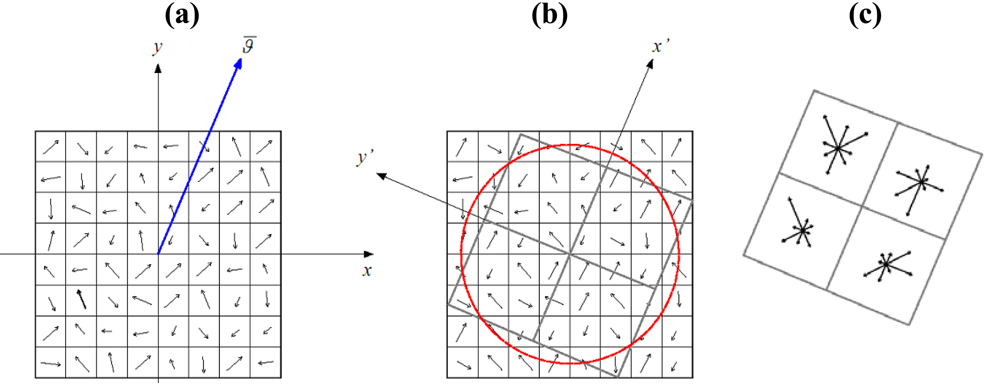
\includegraphics[width=.8\textwidth]{img/rotationDescriptorfinal.png}
\end{frame}

\begin{frame} {Feature Descriptor}
\begin{itemize}
	\item  4x4 arrays of 8 bin histogram is used
	\item  a total of 128 features for one keypoint
\end{itemize}
%  \begin{itemize}
%  4\times4 arrays of 8 bin histogram is used, this is a 128 dimensional vector
%  \item a total of 128 features for one keypoint
%  \end{itemize}
 % \begin{tabular}{cc}
 %   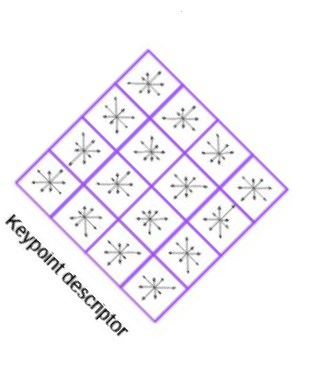
\includegraphics[width=.2\textwidth]{img/KeypointDescriptor.png}
 %   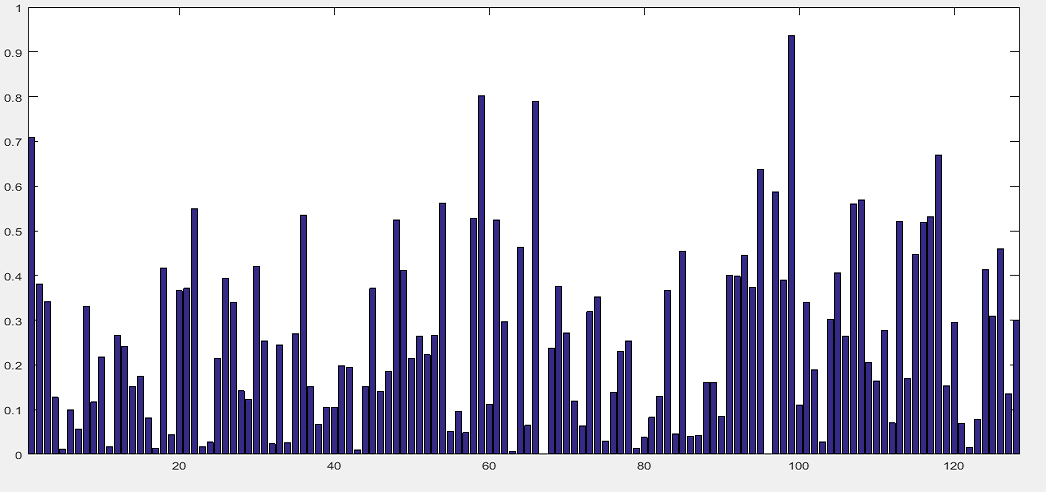
\includegraphics[width=.2\textwidth]{img/hist_rand.png}
 % \end{tabular}
  \begin{columns}
    \begin{column}{.4\textwidth}
      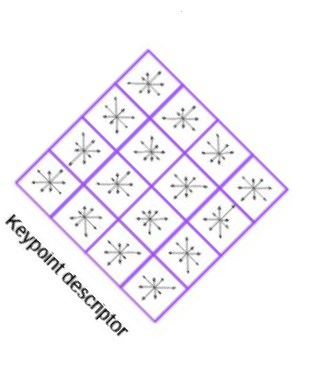
\includegraphics[width=.7\textwidth]{img/KeypointDescriptor.png}
    \end{column}
    \begin{column}{.6\textwidth}
      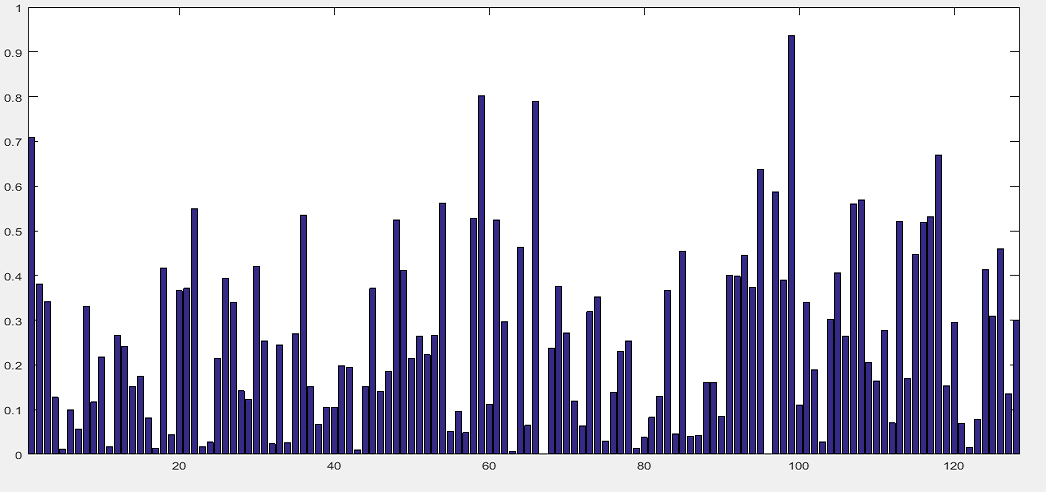
\includegraphics[width=.7\textwidth]{img/hist_rand.png}
    \end{column}
  \end{columns}
\end{frame}

\subsection{SURF}
\begin{frame}{SURF(Speed Up Robust Feature)}
	\begin{itemize}
		\item \textbf{Scale Space:} In SURF, square-shaped filters are used as an approximation of Gaussian smoothing.
		\item \textbf{Key point detection:}Hessian matrix and Non-maximum suppression.
		\item \textbf{Orientation:}Sliding orientation window using Gaussian weighted Haarwavelet responses from circular neighborhood
		\item \textbf{Descriptor:}An oriented 4x4 grid that defines subregion. Wavelet responses computet for 5x5 samples of the subregion.

	\end{itemize}
\end{frame}
\subsection{PHOW}
\begin{frame}{PHOW}
	The PHOW features are a variation of dense SIFT descriptors, extracted at multiple scales. A color version, extracts descriptors on the three color channels and stacks them up.
	\begin{itemize}
		\item When computing descriptors for many keypoints differing only by their position (and with null rotation), further simplifications are possible.
	\end{itemize}
		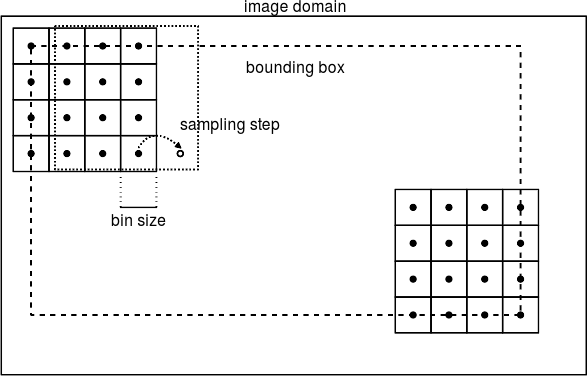
\includegraphics[width=8cm,height=4cm]{img/dsift.png}
\end{frame}


\subsection{ORB}
\begin{frame}[t]{ORB(Oriented FAST and Rotated BRIEF)}
	\begin{itemize}
		\item FAST used to find key-points.
		\item Unlike the orientation operator in SIFT, which can have multiple value on a single keypoint, the centroid operator gives a single dominant result.
		\item Dimensionality reduction can be achieved by using hash functions that reduce SIFT descriptors to binary strings
	\end{itemize}
	
	\begin{columns}
	\begin{column}{.4\textwidth}
	\begin{block}{Corner Detection}
	A corner is detected if \textbf{n} contiguous pixels in the circle are brighter or darker than the pixel in the center
	\end{block}
	
    \end{column}
    \begin{column}{.6\textwidth}
		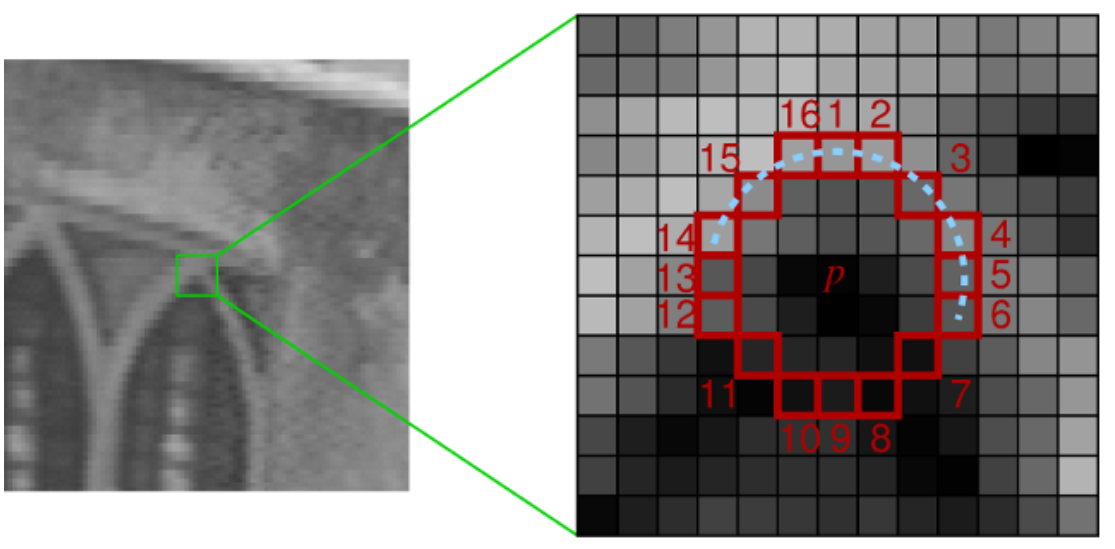
\includegraphics[width=\textwidth]{img/fast.png}
    \end{column}
	\end{columns}
	
\end{frame}

\section{Results}
\subsection{Mean Average Precision}

\begin{frame} {MAP over Ratio}
\tikzoverlay[text width=0.98\paperwidth] at (1cm,3cm) {
	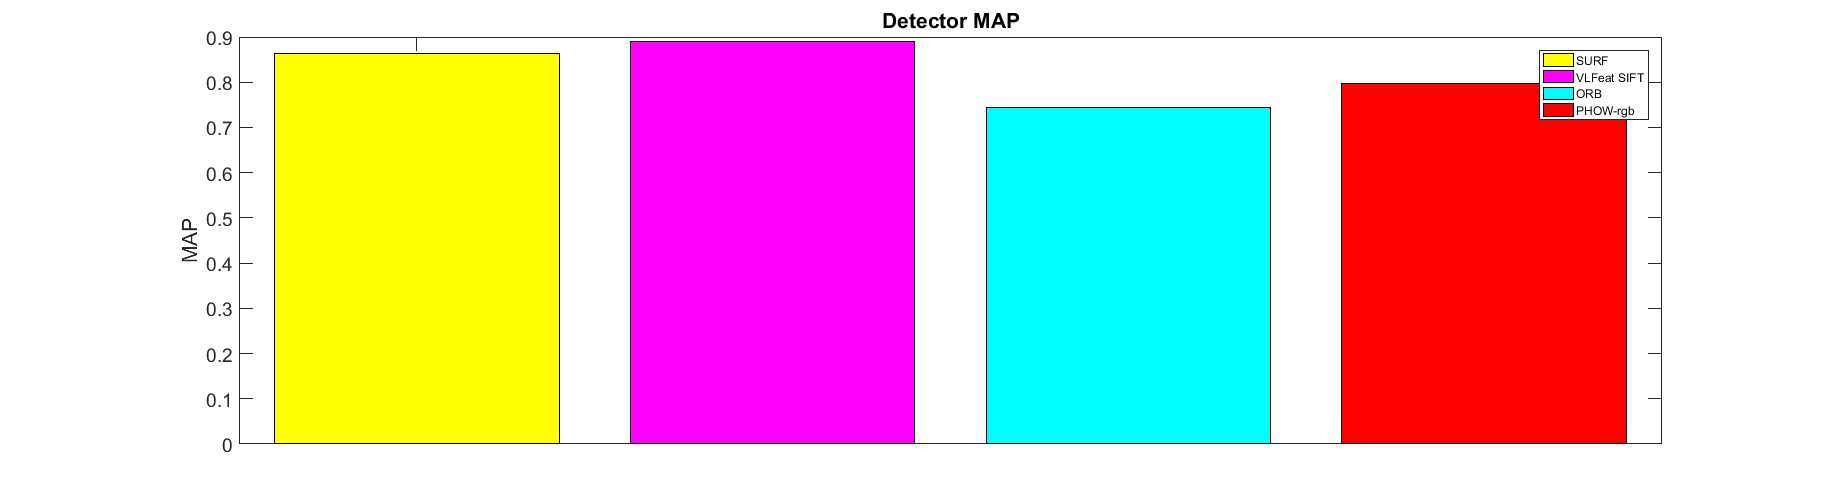
\includegraphics[width=0.6\textwidth]{img/refmap.png}
};
\tikzoverlay[text width=0.98\paperwidth] at (-1cm,1cm) {
  \begin{tabular}{ccc}
	JPEG & 	JPEG XR & JPEG 2000 \\
	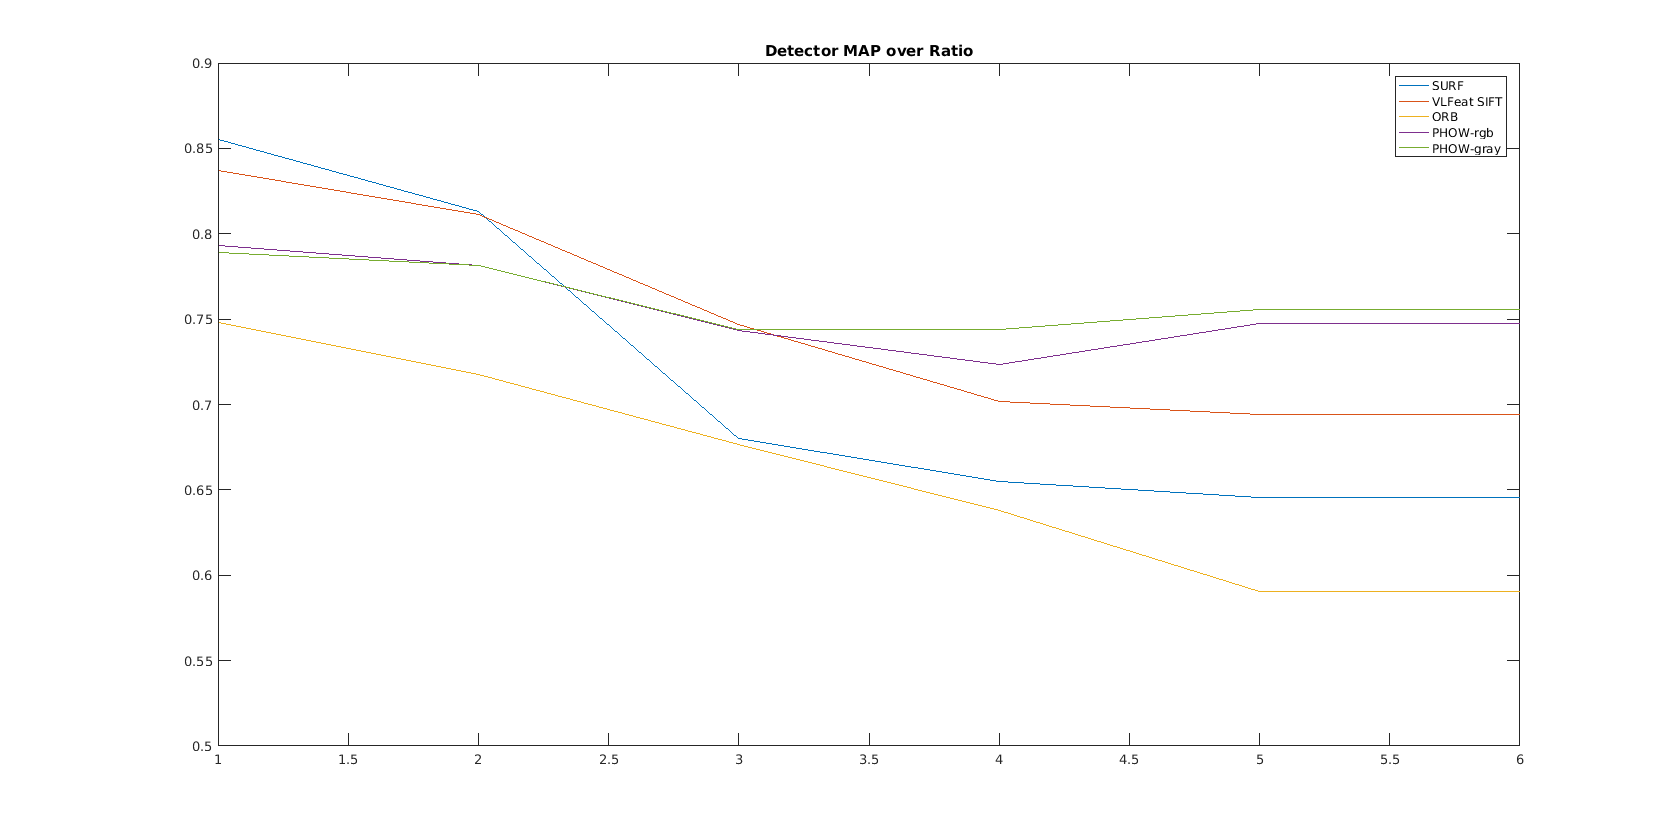
\includegraphics[width=0.3\paperwidth,height=2.9cm]{img/jpg_map.png}&
	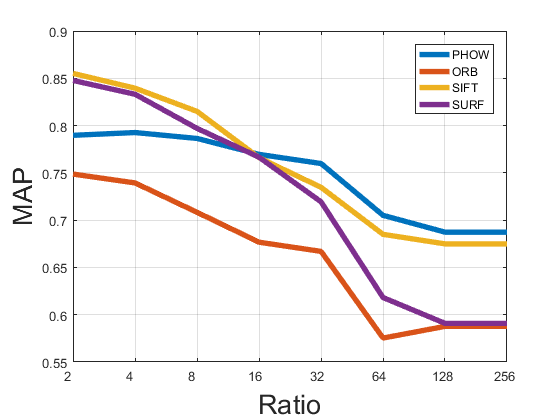
\includegraphics[width=0.3\paperwidth]{img/jxr_map.png}&
	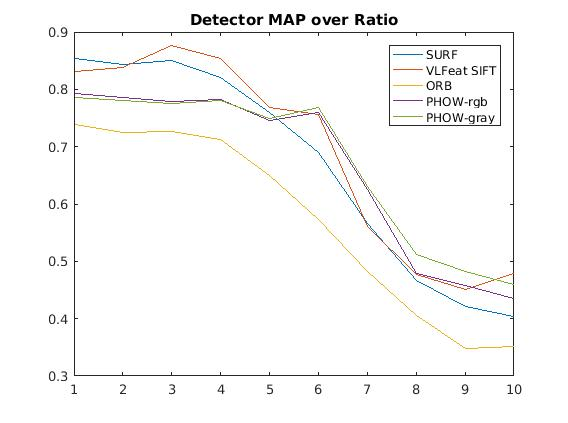
\includegraphics[width=0.3\paperwidth]{img/jp2_map.jpg}\\
  \end{tabular}
};
\end{frame}

\subsection{Query Average Precision}
\begin{frame} {SIFT Query AP over Ratio}
\tikzoverlay[text width=0.98\paperwidth] at (-0.8cm,1cm) {
	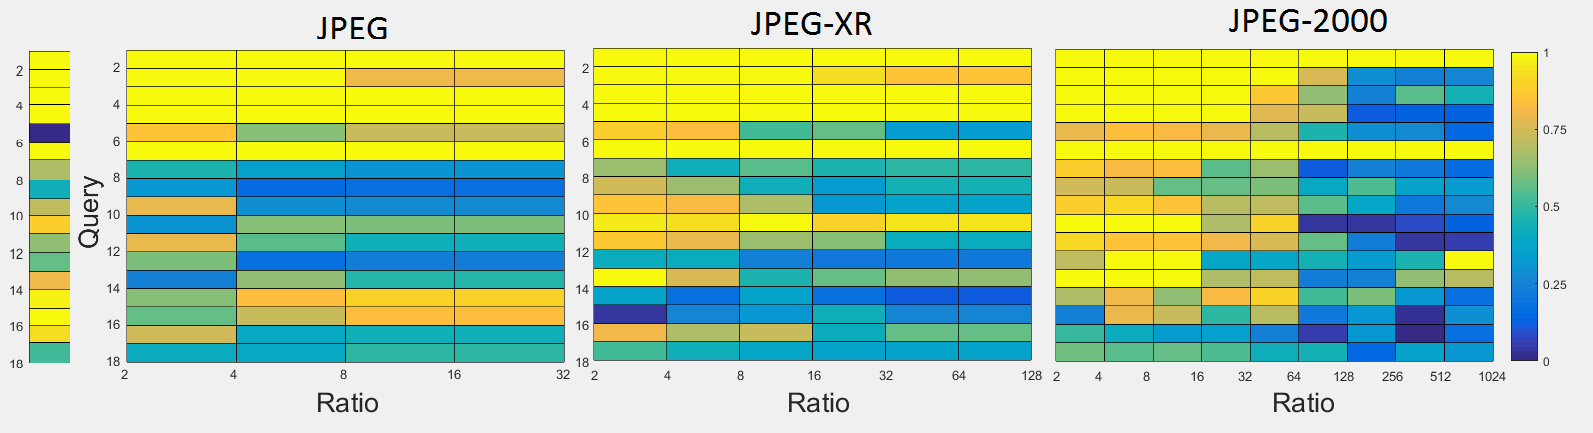
\includegraphics[width=0.97\textwidth]{img/siftqap.png}
	};
\end{frame}

\begin{frame} {SURF Query AP over Ratio}

\tikzoverlay[text width=0.98\paperwidth] at (-0.8cm,1cm) {
	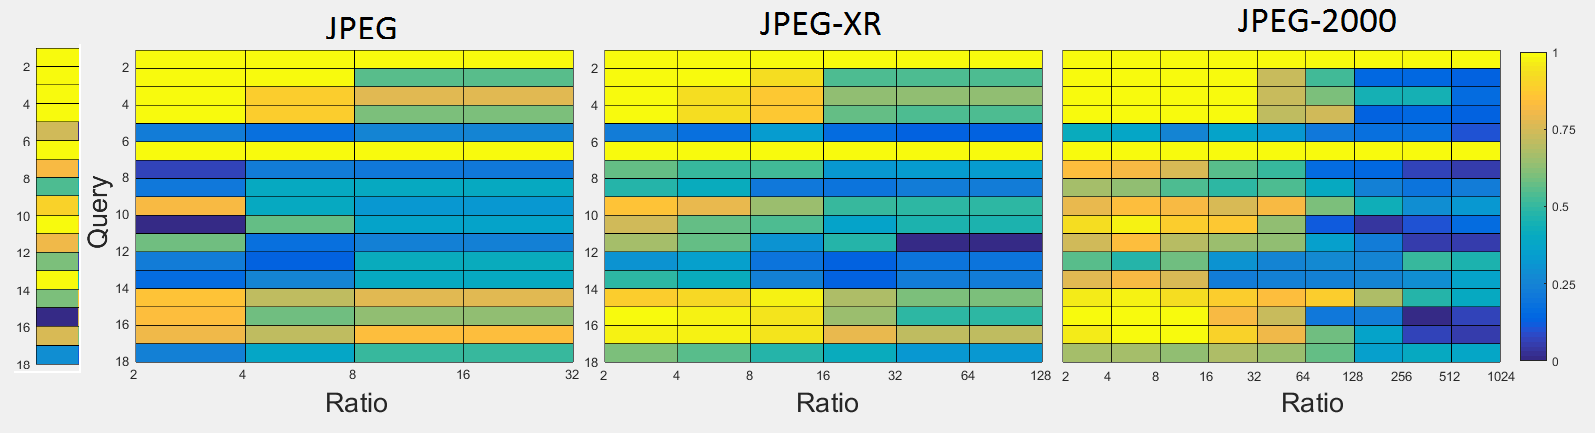
\includegraphics[width=0.95\paperwidth]{img/surfqap.png}
	};
\end{frame}

\begin{frame} {ORB Query AP over Ratio}

\tikzoverlay[text width=0.98\paperwidth] at (-0.8cm,1cm) {
	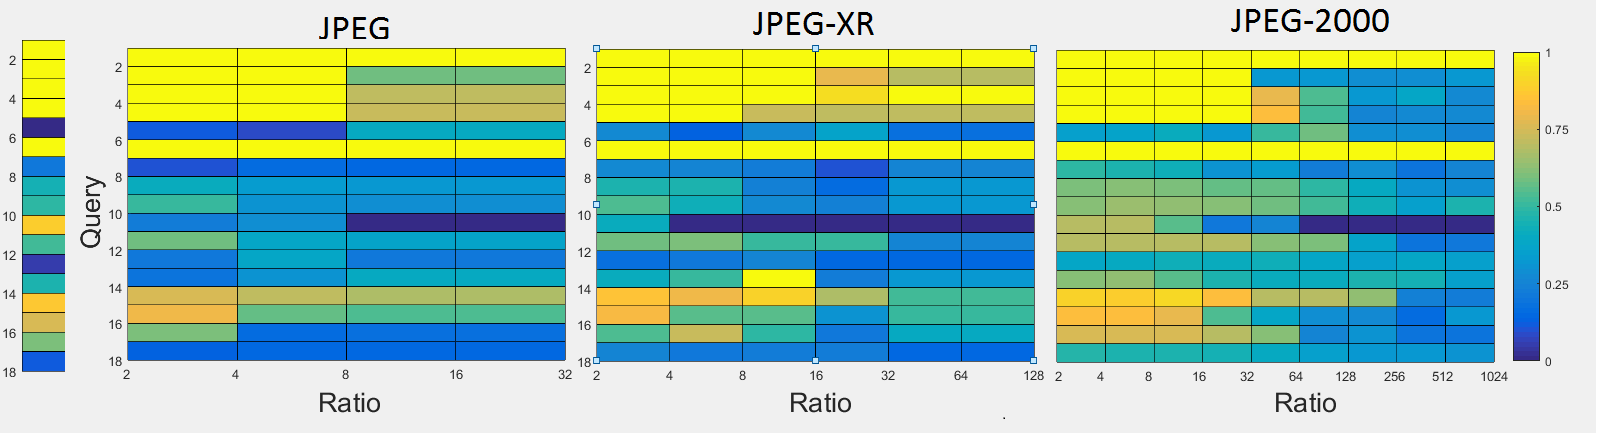
\includegraphics[width=0.95\paperwidth]{img/orbqap.png}
	};
\end{frame}

\begin{frame} {PHOW Query AP over Ratio}
\tikzoverlay[text width=0.98\paperwidth] at (-0.8cm,1cm) {
	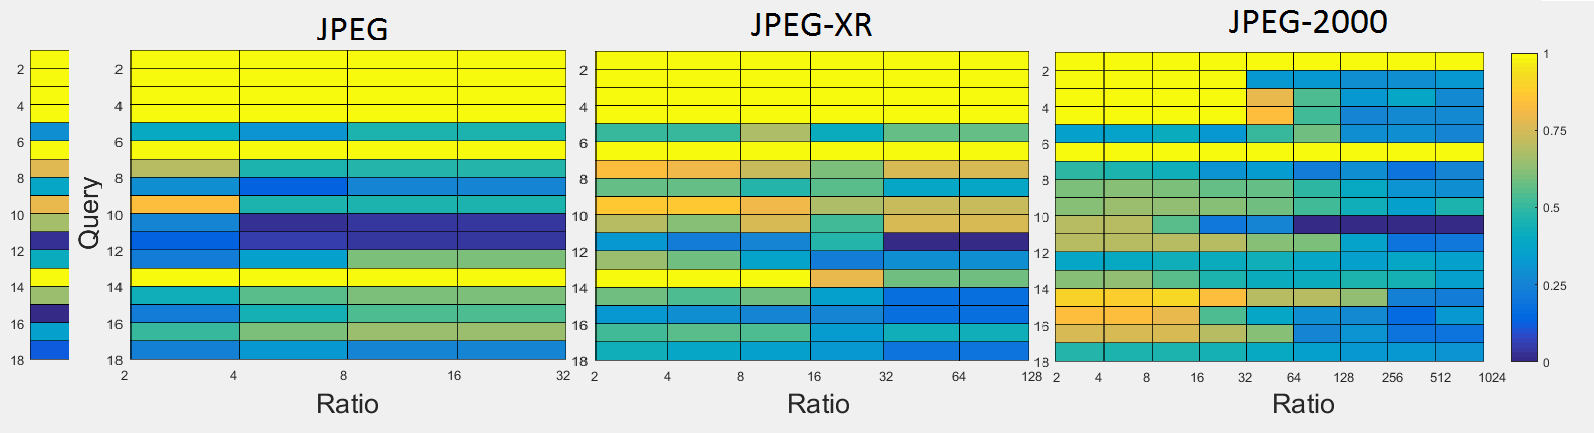
\includegraphics[width=0.95\paperwidth]{img/phowqap.png}
	};
\end{frame}


\subsection{Precision Recall Curve}
\begin{frame} {SIFT PRC over Ratio}
\tikzoverlay[text width=0.98\paperwidth] at (-0.8cm,1cm) {
	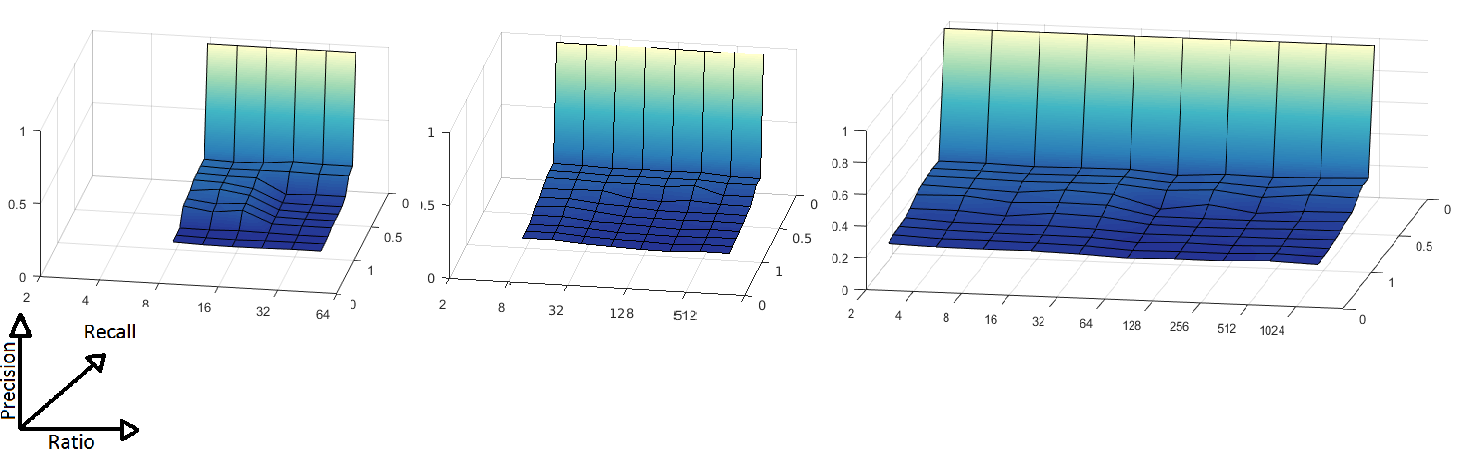
\includegraphics[width=0.95\paperwidth]{img/siftprc.png}
	};
\end{frame}

\begin{frame} {SURF PRC over Ratio}
\tikzoverlay[text width=0.98\paperwidth] at (-0.8cm,1cm) {
	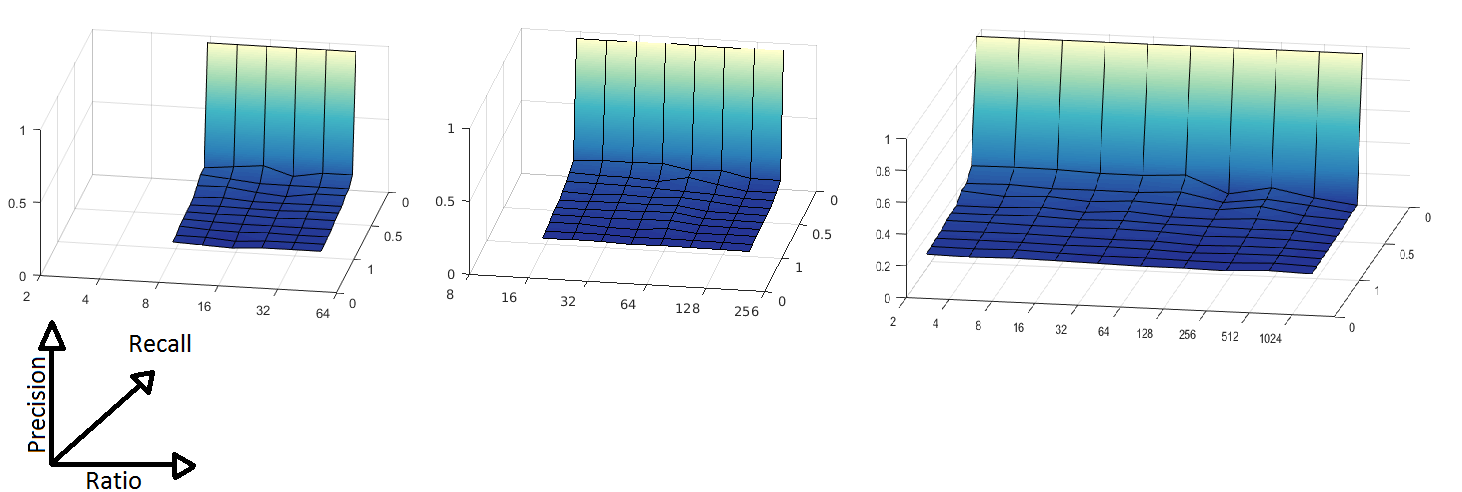
\includegraphics[width=0.95\paperwidth]{img/surfprc.png}
	};
\end{frame}

\begin{frame} {ORB PRC over Ratio}
\tikzoverlay[text width=0.98\paperwidth] at (-0.8cm,1cm) {
	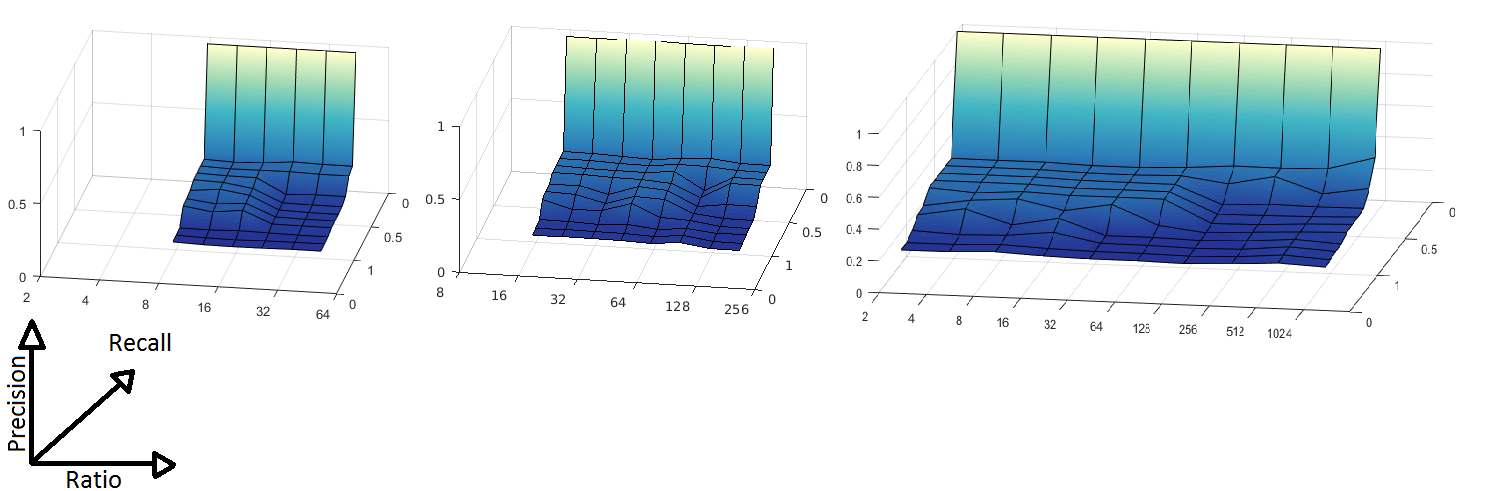
\includegraphics[width=1\textwidth]{img/orbprc.png}
	};
\end{frame}

\begin{frame} {PHOW PRC over Ratio}
\tikzoverlay[text width=0.98\paperwidth] at (-0.8cm,1cm) {
	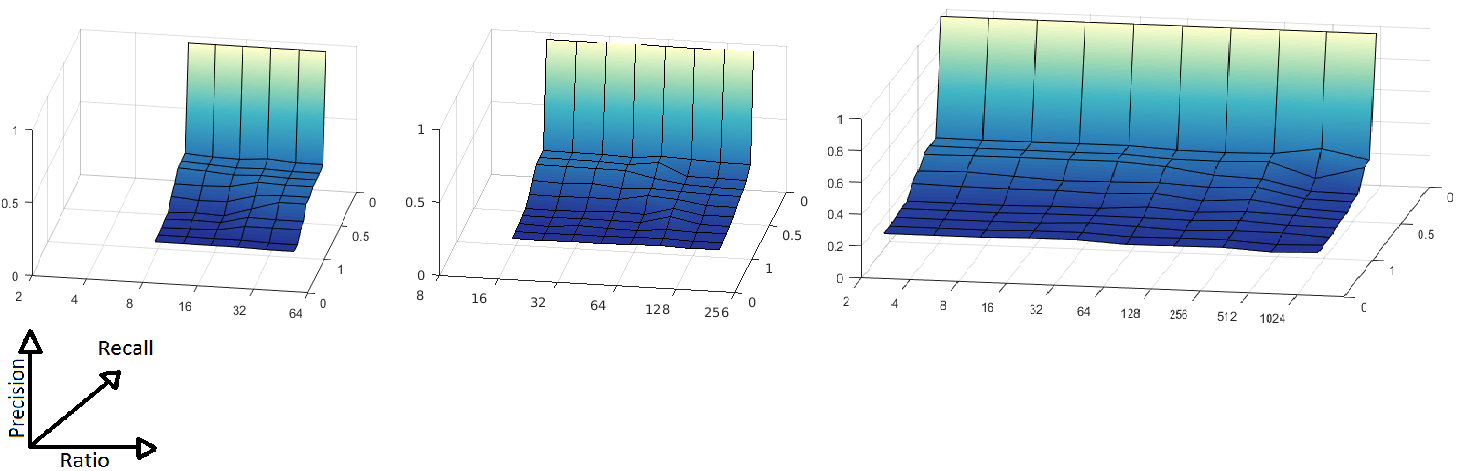
\includegraphics[width=0.95\paperwidth]{img/phow.png}
	};
\end{frame}


\end{document}
